\scanpage{33}
% archive sheet number: 32

\margin{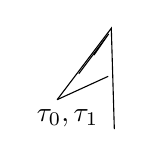
\begin{tikzpicture}[scale=.55]\draw (0,0)--(1.25,1.65)--(1.32,-.68);\draw (0,0)--(1.18,.54);\node[below] at (.24,0) {\deleted{$\unsure{\tau_0,\tau_1}$}};\draw (.5,.6)--(1.19,1.52)--(.85,1.03);\end{tikzpicture}}
\[
(V,\deleted{\unsure{f_0}}f_V,\{L_i\}_{0\leq i\leq n},a_0\}
\]

$V$ fibré vectoriel rang $n+1$

$f_V$ forme quadratique

$L_i$ sous-fibré vectoriel rg $1$\qquad $0\leq i\leq n$

$a_0$ \deleted{base} \inserted{section} de $L_0$ \deleted{(rigidification \ldots)}

a) $f_V|L_i$ lisse \deleted{[\unsure{et $\varphi|L_i$ est non dégénérée en tte fibre, en ce sens}]} $0\leq i\leq n$

b) $L_i\perp L_j$ si $0\leq i<j\leq n$ \quad $j,\deleted{\unsure{\leq|\ne}},i$ non consécutifs

c) $L_i\not\perp L_{i+1}$ sur \deleted{aucune} \inserted{tte} fibre $(0\leq i\leq n-1)$

d) $f(a_0)=1$ (normalisation pour $L_0$ et $f$ ]

Correspond aux \unsure{$n$-polyèdres|hyperpolyèdres} réguliers \unsure{pseud.|pseudo.} épinglés pour lesquels $\beta=\prod\beta_i$ inversible (mais $\widetilde\rho$ pas néc. inv, i.e. $f_V$ pas néc. lisse \ldots)

\diagram{\begin{tikzcd}[ampersand replacement=\&,column sep=.55em,row sep=1.7em]
\deleted{L_0}\arrow[dr,dash,"{\deleted{\tau_0}}"']\&\deleted{\unsure{L_1}}\arrow[d,dash]\&{}\&L_0\arrow[dl,dash,"{\tau_0}"']\arrow[dr,dash,"{\unsure{1|\tau_0}}"]\&{}\&L_1\arrow[dl,dash,"{\tau_1}"']\arrow[dr,dash]\&{}\\
{}\&\deleted{L'_0}\&L'_0\&{}\&L'_1\&{}\&L'_2
\end{tikzcd}\quad
\begin{tikzcd}[ampersand replacement=\&,column sep=.6em,row sep=1.7em]
{}\&L_i\arrow[dl,dash,"{\tau_i}"']\arrow[dr,dash,"{\unsure{1|\tau_i}}"]\&{}\&L_{i+1}\arrow[dl,dash]\\
L'_i\&{}\&L'_{i+1}\&{}
\end{tikzcd}\quad$\big|\,\beta_i$}

\[
L'_i=\psi_V(L_i)
\]

\[
\boxed{\varphi(a_i,a_{i+1})=-f(a_{i+1})}\ \text{\uline{inv.}}
\]
définit de proche en proche les \uline{bases} $a_i$ des $L_i$, à partir de $L_0$ déjà donnée

\[
a_i\in L_i\qquad\mathord{\tikz[baseline=(q.base)]{\node[inner sep=1pt] (q) {$a'_{i+1}=\psi(b_{i+1})$};\draw (q.center) ellipse (1.63cm and .38cm);}}
\]
\[
\langle a_i,a'_{i+1}\rangle=1\quad\text{i.e.}\quad \boxed{\varphi(a_i,b_{i+1})=1}
\]
\[
\deleted{a_{i+1}a'_{i+1}}\qquad
\mathrm{id}+\underbrace{a'_{i+1}}_{\deleted{\psi(b_{i+1})}}\otimes a_{i+1}=\tau_{i+1}
\]
\[
\left\{\begin{aligned}
a_{i+1}&=\unsure{\zeta_{i+1}|\gamma_{i+1}|\xi_{i+1}}b_{i+1}=\frac{-1}{f(b_{i+1})}b_{i+1}\\
\zeta_{i+1}&=-f(a_{i+1})\deleted{\unsure{\zeta_i|\xi_i|b_i}}=-\frac1{f(b_{i+1})}\\
&=-\zeta_{i+1}^2 f(b_{i+1})
\end{aligned}\right.
\]
\[
1=-\zeta_{i+1}f(b_{i+1})
\]
\[
\begin{aligned}
a'_{i+1}&=\frac{-1}{f(a_{i+1})}\psi(a_{i+1})\\
&=\psi\left[\underbrace{-\frac1{f(a_{i+1})}a_{i+1}}_{b_{i+1}}\right]\\
&\deleted{\unsure{\text{d'où }|b_{i+1}=}a_{i+1}=-\frac1{f(\unsure{a})}}
\end{aligned}
\]
\[
\varphi(a_i,a_{i+1})=\frac{1}{\deleted{\unsure{a_{i+1}}}}\zeta_{i+1}=-f(a_{i+1})
\]
